
\begin{figure*}
\begin{center}
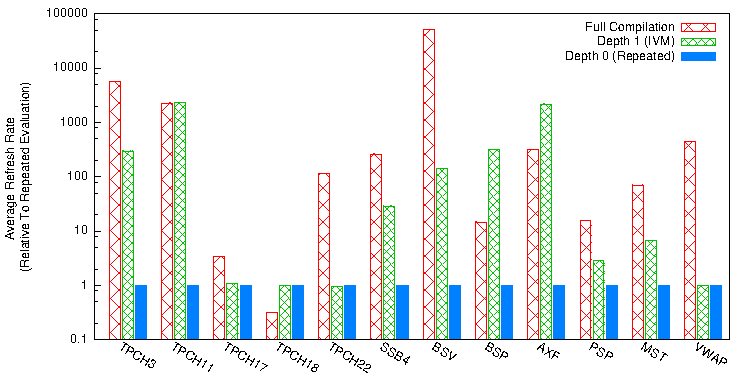
\includegraphics[width=\textwidth]{../graphs/graphs/bakeoff.pdf}
\caption{Cross-query comparison of our compiler in different depth-restricted modes, and the best performing streaming and database engine for each query.  Note the logscale on the y-axis.}
\label{fig:experiments:bakeoff}
\end{center}
\end{figure*}

We now analyze the performance of our compilation techniques.  As in Section \ref{sec:dbfail}, our experiments are run on Redhat Enterprise Linux running in a VM with 16 GB of RAM, and 2x4 core Intel Xeon E5620 2.4 GHz processors allocated to it.  Note that our compiler produces single-threaded code, while other platforms were allowed to consume the full resources of the VM.
 
Our analysis uses the queries from Examples \ref{ex:dbfail:stock}(PRICESPREAD),  \ref{ex:dbfail:tpch}(SHIPPING), and \ref{ex:dbfail:network}(SERVERLOAD), Queries numbers 3, 11, 17, 18, and 22 from the TPC-H\cite{tpch} benchmark, the VWAP query presented in \cite{kennedy-ahmad-koch-cidr:11}, and four additional financial queries: MISSEDTRADES, AXFINDER, BROKERSPREAD, and BROKERCOVARIANCE in the spirit of VWAP and PRICESPREAD.  The structure of these queries is described below.

Queries were run on pre-generated traces until completion of the trace or a 1 hour cutoff.  Traces are implemented as follows: The queries: VWAP, MISSEDTRADES, AXFINDER, BROKERSPREAD, PRICESPREAD, and BROKERCOVARIANCE were run on a 2.63 million tuple trace of one day of stock market activity for MSFT.  BID and ASK orders (and cancellations) were translated into equivalent operations on a BIDS and ASKS table, with tuples in either table comprised of a timestamp, an order id, a broker id, a price, and a volume.  The broker id was synthesized for each order -- our experiments use 10 brokers, assigned deterministically based on the order id.  The stream consists of approximately 1.4 million operations on the BIDS table, and 1.14 million operations on the ASKS table.

The TPCH-H and SHIPPING queries were run on a database generated by dbgen\cite{tpch} with scaling factor 0.1 (100 MB).  Additional experiments were carried out on TPC-H queries 3, 11, and 22 with a scaling factor 1 (1GB) database.  The results for these queries are presented in Section \ref{sec:experiments:bigds}.  Insertions are drawn from the data files for each table and interleaved in random order.  Note that this means that some insertions are performed before the foreign key that they reference, and that smaller datafiles finish earlier.  Although this is not expected behavior in a streaming setting, it serves to provide valuable insights about the difference between the performance characteristics of different types of insertions.  The size of each stream is as documented in the TPC-H specification\cite{tpch}.

The SERVERLOAD query was run on a synthetically generated dataset, simulating 1000 racks of 20 servers each, followed by 100,000 state updates.  Each server is assigned a rack id and a current load.  The first 20,000 operations in the trace consist of an insertion for each server at 0 load.  Each state update is represented by a random server deleting its previous state tuple, and inserting a new tuple containing a load selected randomly between 0 and 1.  Each state update involves of two table operations, so the stream consists of 220,000 operations.

For comparison, we use a depth-limited instantiation of our compilation algorithm where maps are not materialized beyond a fixed number of recursive steps.  Compilation limited to depth-1 is approximately equivalent to traditional IVM techniques, while depth-0 is equivalent to re-evaluating the query on every insertion\footnote{We have implemented an in-memory query processing engine to support depth-1 and depth-0 compilation.  Although the capabilities of this engine are limited, we do not expect further optimizations  to have a meaningful impact on the processing times of our test queries.}.  We omit detailed depth-0 performance measurements on graphs where these results are not visible due to scale, or where depth-0 and depth-1 performance are indistinguishable.  Memory measurements are taken using google-perftools\cite{perftools} and count only memory allocated to the persistent maps.

Note that we able to take advantage of the TPC-H benchmark's append-only nature: The SHIPPING and the TPC-H queries are compiled without deletion triggers.  As a further optimization, all queries involving strings use a dictionary to compress string data before processing.

\subsection{Equijoins}

\begin{figure}
\begin{center}
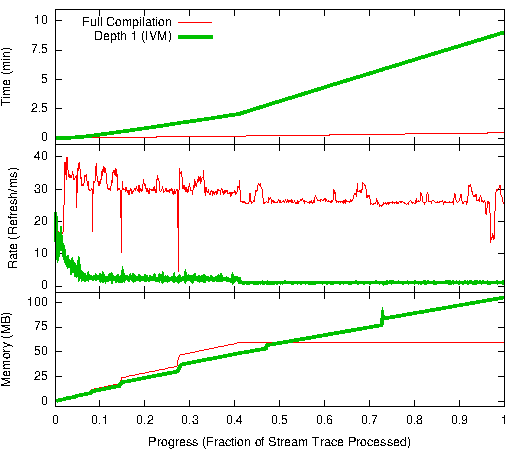
\includegraphics[width=3.4in]{../graphs/graphs/unified_tpch3.pdf}
\caption{Performance comparison on TPC-H Query 3.  Note not only the improved performance of full compilation, but also the relative memory usage of both instantiations.  All streams except LINEITEM have completed by the 40\% marker and insertions into LINEITEM do not consume any additional memory.}
\label{fig:experiments:tpch3}
\end{center}
\end{figure}

\begin{figure}
\begin{center}
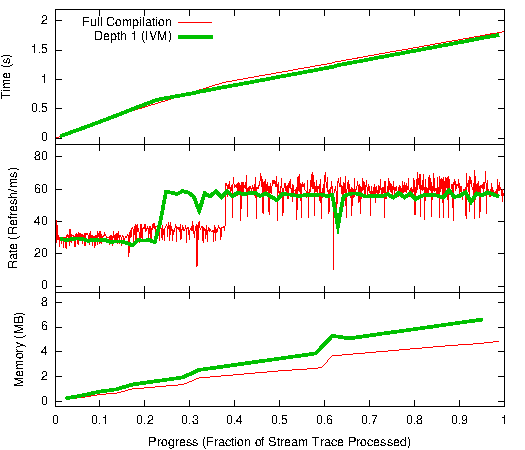
\includegraphics[width=3.4in]{../graphs/graphs/unified_tpch11.pdf}
\caption{Performance comparison on TPC-H Query 11.  The two techniques perform similarly, because for a two-way join full compilation only requires a single recursive step, and fixed (and small) size aggregation.}
\label{fig:experiments:tpch11}
\end{center}
\end{figure}

\begin{figure}
\begin{center}
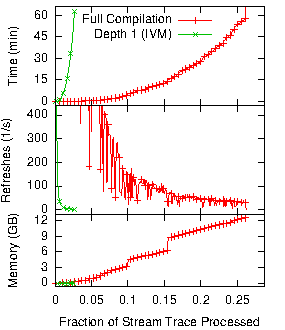
\includegraphics[width=3.4in]{../graphs/graphs/unified_ssb4.pdf}
\caption{Performance comparison on SHIPPING.  Full compilation is a full polynomial order faster than in IVC.  These improvements come at the cost of memory, and performance does begin to drop once the system begins running out of memory at the 27\% marker.}
\label{fig:experiments:ssb4}
\end{center}
\end{figure}

We first analyze the performance of our compiler on three equijoin queries built on the TPC-H benchmark .  TPC-H Query 3 (Figure \ref{fig:experiments:tpch3}) is a 3-way select-project-join-aggregate.  TPC-H Query 11 (Figure \ref{fig:experiments:tpch11}) is the simplest query of the three, a 2-way equi-join on a one-to-many relationship (SUPPLIER to PARTSUPP) with bounded fanout.  SHIPPING (Figure \ref{fig:experiments:ssb4}) is a 7-table join with a join-width of 6.  

Our compiler recurses only once on TPC-H Query 11.  As a consequence, the result is nearly equivalent to IVM\footnote{We pre-aggregate the materializations of SUPPLIER and PARTSUPP, but this is only a minor improvement in practice due to the bounded fanout of this query.}.  

Both TPC-H Query 3 and SHIPPING demonstrate a substantial performance increase over IVM.  The one-to-one, and bounded fanout one-to-many relationships between elements of many of these queries are actually advantageous to the IVM implementation -- each insertion only triggers a limited number of reads.  In spite of this, incrementally maintaining the (aggregate) delta queries results in a net reduction in the amount of work required -- especially in a large query like SHIPPING.

Also note the memory usage of TPC-H Query 3.  During the final stretch starting by the 40\% marker, the all streams have been exhausted except for LINEITEM.  The final aggregate's group-by columns are drawn purely from the order table, so insertions into LINEITEM only update aggregate values that were already  allocated by the corresponding ORDER.  Consequently, memory usage plateaus for full compilation, while the IVM implementation must continue to store each row.

This is not always true.  For extremely large queries like SHIPPING (a 7-way join), the number of intermediate datastructures created is quite large.  In spite of the large amount of state that the fully compiled query maintains, the amount of state modified per update is small and the fully compiled query's efficiency is unaffected as long as the system has enough memory.  Even so, memory usage is an important part of the cost/benefit tradeoff of full compilation, and is explored in greater detail below, in Section \ref{sec:experiments:othermetrics}.

\subsection{Nested Subqueries}

\begin{figure}
\begin{center}
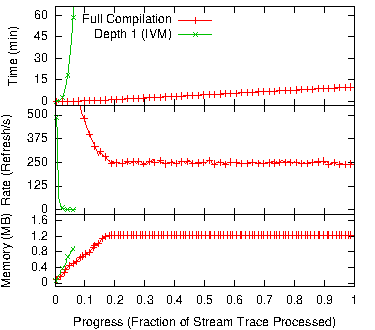
\includegraphics[width=3.4in]{../graphs/graphs/unified_tpch22.pdf}
\caption{Performance comparison on TPC-H Query 22.  Execution of the IVM implementation was terminated after 60 minutes.  The much smaller CUSTOMERS stream completes around the 18\% marker, leaving only the O(1) insert cost of insertions into ORDERS.  Each insertion into ORDERS only updates a per-customer aggregate, and consumes no additional memory.}
\label{fig:experiments:tpch22}
\end{center}
\end{figure}

\begin{figure}
\begin{center}
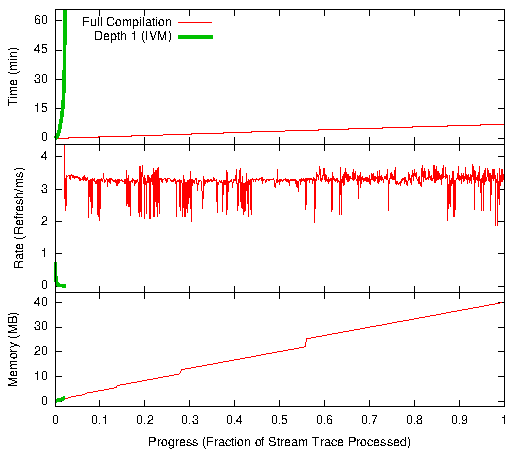
\includegraphics[width=3.4in]{../graphs/graphs/unified_vwap.pdf}
\caption{Performance comparison on VWAP.  Execution of the IVM implementation was terminated after 60 minutes.  The IVM implementation must repeatedly re-evaluate a correlated nested subquery, while the fully compiled version incrementally maintains pre-computed versions of the query for a fixed domain of already encountered values.  The unbounded memory growth is discussed in Section \ref{sec:experiments:future}.}
\label{fig:experiments:vwap}
\end{center}
\end{figure}

\begin{figure}
\begin{center}
%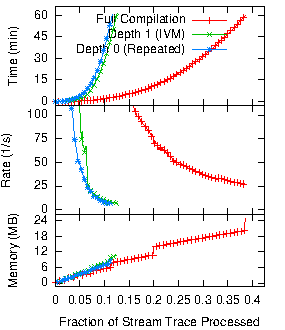
\includegraphics[width=3.4in]{../graphs/graphs/unified_tpch17.pdf}
\caption{Performance comparison on TPC-H Query 17}
\label{fig:experiments:tpch17}
\end{center}
\end{figure}

\begin{figure}
\begin{center}
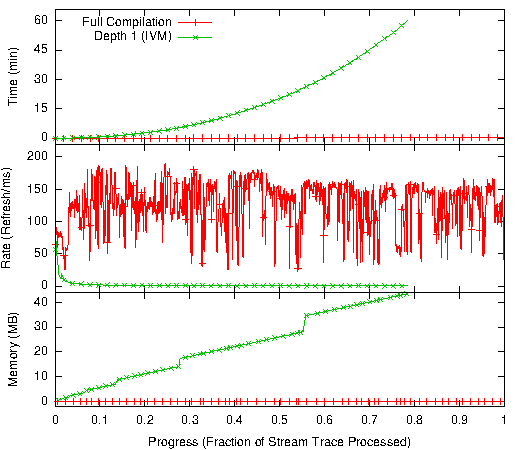
\includegraphics[width=3.4in]{../graphs/graphs/unified_brokervariance.pdf}
\caption{Performance comparison on BROKERCOVARIANCE.  Execution of the IVM implementation was terminated after 60 minutes.  Although this is a 2-way join like TPCH Query 11, the join relationship is many-to-many and requires a linear amount of work in IVM.  Conversely, the fully compiled version stores only the aggregate results and requires a constant amount of work for each insertion.}
\label{fig:experiments:brokervariance}
\end{center}
\end{figure}

Figures \ref{fig:experiments:tpch22}, \ref{fig:experiments:vwap}, and \ref{fig:experiments:tpch17} illustrate the performance of our compiler on several queries with nested aggregates.

Of these, TPC-H Query 22 queries the CUSTOMER table with two selection conditions: a comparison based on an uncorrelated nested aggregate query over CUSTOMER, and a second based on a lookup (an EXISTS) on ORDERS.  The lookup over orders can be evaluated in constant time both using IVM and full compilation.  However each insertion into ORDERS requires evaluation of the nested aggregate on CUSTOMER, while this value is materialized by the fully compiled version.  

In IVM, insertions into CUSTOMER depend on whether the query optimizer detects that the nested aggregate is uncorrelated and computes it before the rest of the query.  If not, the insertion requires quadratic work, and even if it does, each insertion requires two complete iterations over the customer table: once to compute the aggregate and once to figure out for which customers the state of the comparison changes.  This latter iteration can not be eliminated by full compilation, but the iteration is only over those rows already known to satisfy the selection condition on ORDERS.

VWAP is a query over BIDS with two selection predicates: one over an uncorrelated nested aggregate over BIDS, and one over a correlated (via inequality on the price from the outer BIDS table) nested aggregate over BIDS.  As in TPC-H Query 22, whether the uncorrelated aggregate is an issue for IVM is dependent on the query optimizer.  

The inequality-correlated aggregate is of more interest here.  Because the domain of the correlating variable (price) is determined outside the nested aggregate, the nested subquery must be re-evaluated every time a new price is encountered.  However, the resulting value can then be stored and incrementally maintained.  The domain of prices is bounded, so after an initial ramp up process (that occurs while the size of the table is small) the fully compiled version can incrementally maintain the query output in (close to) constant time.

BROKERCOVARIANCE (Figure \ref{fig:experiments:brokervariance}) is a two-way aggregate self-equi-join over BIDS.  Despite the lack of a nested aggregate, the performance of BROKERCOVARIANCE follows a pattern similar to the prior two queries.  This is not surprising -- correlated aggregate subqueries are known to be equivalent\todo{cite?} to joining the result with a group-by aggregate query.  Thus, materializing a nested aggregate is tantamount to materializing the first delta.  Furthermore, unlike TPC-H Query 11 (Figure \ref{fig:experiments:tpch11}), the join relationship is many-to-many, and the benefits of maintaining the join result as an aggregate grow over time.

TPC-H Query 17 is a two-way equi-join over PART and LINEITEM with a correlated nested aggregate over LINEITEM.  Both the join and the correlation are on partkey.  As in the prior queries in this section, incrementally maintaining the nested aggregate makes insertions into PART constant-time rather than linear.  However, even in the fully compiled query, insertions into the LINEITEM table must still iterate over all matching results in the join, which are already being materialized.  

\subsection{A Bigger Dataset}
\ref{sec:experiments:bigds}

\todo{run experiments}

\subsection{Memory, Extraction, and Future Work}
\label{sec:experiments:future}
\begin{figure}
\begin{center}
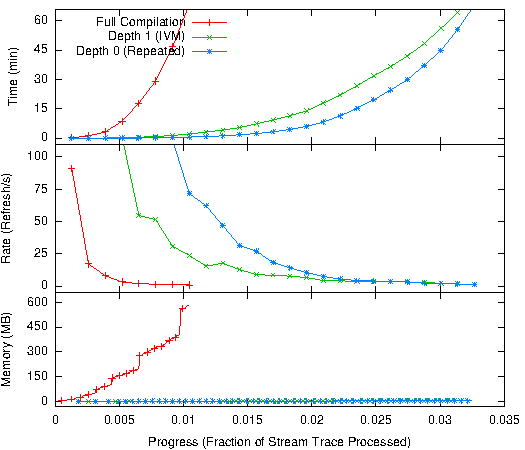
\includegraphics[width=3.4in]{../graphs/graphs/unified_tpch18.pdf}
\caption{Performance comparison on TPC-H Query 18.  An incorrectly chosen join ordering prevents us from effectively exploiting foreign key dependencies in the TPC-H schema, and results in both unnecessary work and the unnecessary extension of an intermediate datastructure's domain.}
\label{fig:experiments:tpch18}
\end{center}
\end{figure}

\begin{figure}
\begin{center}
%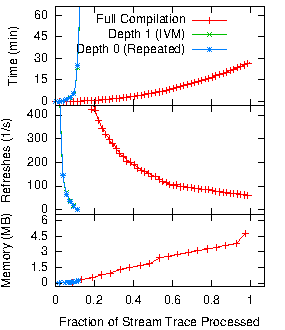
\includegraphics[width=3.4in]{../graphs/graphs/unified_serverload.pdf}
\caption{Performance comparison on SERVERLOAD}
\label{fig:experiments:serverload}
\end{center}
\end{figure}

\begin{figure}
\begin{center}
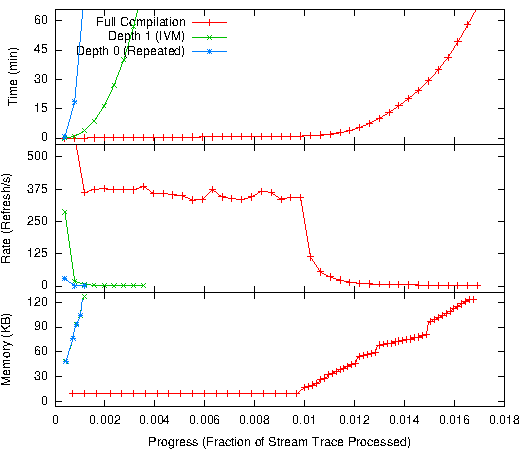
\includegraphics[width=3.4in]{../graphs/graphs/unified_pricespread.pdf}
\caption{Performance comparison on PRICESPREAD.  The performance and memory plateaus result from a portion of the trace from about 0.001\% to 0.01\%, where a single order is repeatedly placed and revoked.}
\label{fig:experiments:pricespread}
\end{center}
\end{figure}

\begin{figure}
\begin{center}
%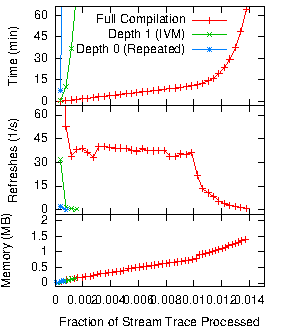
\includegraphics[width=3.4in]{../graphs/graphs/unified_missedtrades.pdf}
\caption{Performance comparison on MISSEDTRADES.  The performance and memory plateaus result from a portion of the trace from about 0.001\% to 0.01\%, where a single order is repeatedly placed and revoked.}
\label{fig:experiments:missedtrades}
\end{center}
\end{figure}


\begin{figure}
\begin{center}
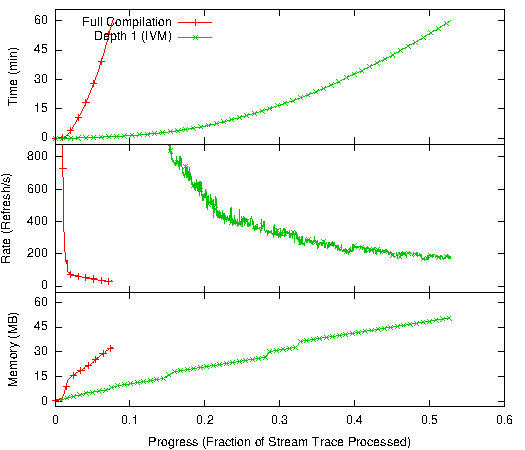
\includegraphics[width=3.4in]{../graphs/graphs/unified_axfinder.pdf}
\caption{Performance comparison on AXFINDER}
\label{fig:experiments:axfinder}
\end{center}
\end{figure}

\begin{figure}
\begin{center}
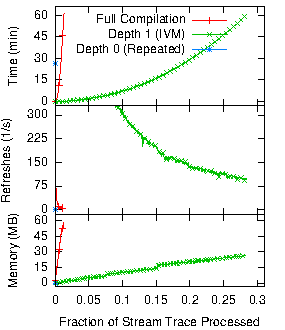
\includegraphics[width=3.4in]{../graphs/graphs/unified_brokerspread.pdf}
\caption{Performance comparison on BROKERSPREAD}
\label{fig:experiments:brokerspread}
\end{center}
\end{figure}

It is important to understand not only where our compiler succeeds, but its limitations of are.  We now consider three cases where the observed performance of our technique does not match up with our expectations, and consider both why the problem occurs and how one might approach a solution.

The first case of poor performance we consider is TPC-H Query 18 (Figure \ref{fig:experiments:tpch18}), a three-way join over CUSTOMER, ORDERS, and LINEITEM, with an EXISTS predicate over a query that itself has a nested aggregate as a condition.  Although the query effectively involves two levels of nesting, it is otherwise quite simple.

Yet in spite of the simplicity, the query performs badly -- the query performs better at depths 0 and 1.  The reason for this poor performance is our join ordering heuristic: The trigger that updates the query result must compute a join between the delta of the extracted nested subquery (aggregated over orderkey) and a materialized representation of CUSTOMER JOIN ORDER JOIN LINEITEM (aggregated over custkey and orderkey).  Not knowing about the one-to-many relationship between custkey and orderkey, we iterate over the materialized join first and effectively iterate over all orders placed so far.  Join ordering is a well studied problem in the database community, and the solution to this problem is purely an engineering challenge (albeit a big one; we have yet to see a stable, publicly available in-memory database engine).  

The second case is best illustrated by SERVERLOAD (Figure\ref{fig:experiments:tpch18}), a query over a single SERVERS table with a single selection predicate based on two uncorrelated aggregates.  By all rights, this query should perform as well as TPC-H 22, VWAP, and BROKERCOVARIANCE (Figures \ref{fig:experiments:tpch22}, \ref{fig:experiments:vwap}, \ref{fig:experiments:brokervariance}).  The difficulty here is related to domain maintenance \todo{Do we discuss this elsewhere in the paper?  Backreference... this is not the place to be discussing it}.  In effect, our runtime is unable to properly garbage collect deleted entries in one of the materialized views, resulting in a progressively growing workload on every insertion.  

A similar issue affects both PRICESPREAD and MISSEDTRADES (Figures \ref{fig:experiments:pricespread}, and \ref{fig:experiments:pricespread}), both two-way joins over BIDS and ASKS.  In both queries there are two selection predictaes: one comparing a column of ASKS to nested subquery over ASKS, and a similar predicate over BIDS.  Apart from a stretch of updates (0.001\% to 0.01\% in the trace) in the stock market trace where the same order is repeatedly placed and revoked -- an apparent denial of service attack or broken automated trading system\footnote{It should be noted that our performance characteristics during the denial of service attack are even better than during normal operations.} -- the query performance follows a very similar performance curve. 

The final case of performance issues is seen in both AXFINDER and BROKERSPREAD, both simple two-way inequality joins.  Our aggressive extraction heuristic attempts to materialize the entire delta query, which for inequality joins includes an unbound variable.  In such cases, the extracted expression is incrementally maintained for every encountered valuation of the unbound variable.  Thus, each change to the extracted expression requires an iteration over all previously encountered values.  In most cases, most of the state kept for each row in this output can be pre-aggregated and is typically quite small.  However, in the case of these two queries, these tables are each approximately the size of both input tables.  An improved, data-dependent extraction heuristic could identify such situations and compute the inequality join inline -- effectively doing what IVM does.  Alternatively, the entire materialized delta could be incrementally maintained more efficiently using datastructures suited to computing aggregates over ranges (e.g., \cite{range trees}).


\subsection{Other Metrics}
\label{sec:experiments:othermetrics}
%\begin{figure}
%\begin{center}
%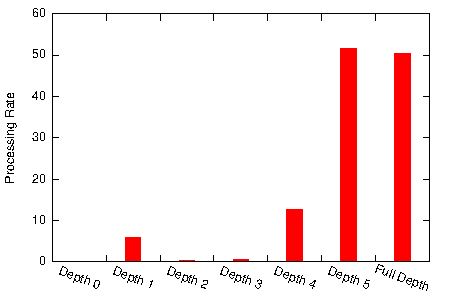
\includegraphics[width=3in]{../graphs/graphs/depth_ssb4.pdf}
%\caption{Average processing rate as a function of compilation depth on SHIPPING.}
%\label{fig:experiments:ssb4depth}
%\end{center}
%\end{figure}

\begin{figure*}
\begin{center}
\begin{tabular}{|l|c|c|c|c|c|c|}\hline
{\bf Depth} & 1 & 2 & 3 & 4 & 5 & Full \\ \hline 
Avg Rate (refreshes/s) & 5.91 & 0.373 & 0.7 & 12.7 & 51.5 & 50.4 \\ \hline 
Avg Memory per Tuple & 98.5 B & 0.0 B & 0.0 B & 0.0 B & 0.0 B & 61.0 KB \\ \hline 
Lines of Code & 3174 & 12015 & 16517 & 13215 & 10998 & 10431 \\ \hline 
Number of Maps &        6 &       18 &       36 &       45 &       45 &       39 \\ \hline 
\end{tabular}
\caption{Statistics for different compilation depths on SSB4.  Depth-5 is equivalent to full compilation, but also maintains copies of each of the 6 base relations.}
\end{center}
\end{figure*}

\tinysection{Limited recursion}
We now explore the space of limited recursive compilation beyond IVM.  Figure \ref{fix:experiments:ssb4depth} illustrates the effects of limiting compilation to depths between 0 and 5.  Recall that the maximum recursive depth is one less than the join width of the query.  Thus for SHIPPING (which has a join width of 6), compilation to depth-5 is approximately equivalent to full compilation.

At depth-1, the compiled query materializes only the base relations and no intermediate tables.  It must still perform a 5-way join on every insertion, but  only once per update.  The 6 datastructures that it maintains are the 6 relations that appear in the query.  

At depth-2, the compiled query must now maintain 12 intermediate datastructures, several of which require (effectively) a 4-way join to maintain.  The net cost of maintaining these additional maps does not begin to pay off until depth-4 (where maintenance operations are reduced to at most 2-way joins).  By this point, decomposition has already resulted in the instantiation of all intermediate materializations relevant to the query, so extra and unnecessary work is being done.  

The effectiveness of this approach at depth-4 (in spite of the extra work being done) suggests that a more effective approach to reducing memory consumption might be to materialize not just the set of datastructures closest to the root, but rather a subset of the entire compilation tree.  However, there exists an incredibly large space of possible materialization plans ($2^{39} \approx $ half a trillion possibilities for SHIPPING), and an effective cost-based materialization plan optimizer is well beyond the scope of this paper.


\begin{figure}
\begin{center}
\begin{tabular}{|l|c|c|c|}\hline 
\ & Infinite Depth & Depth 1 & Depth 0 \\\hline 
TPCH3 & 2509 & 2855 & 4198 \\\hline
TPCH11 & 531 & 596 & 616 \\\hline
TPCH17 & 928 & 1158 & 1478 \\\hline
TPCH18 & 3668 & 3538 & 4631 \\\hline
TPCH22 & 777 & 1135 & 754 \\\hline
SSB4 & 10995 & 8954 & 7904 \\\hline
BSV & 342 & 327 & 347 \\\hline
BSP & 45625 & 567 & 729 \\\hline
AXF & 2169 & 553 & 1394 \\\hline
PSP & 1442 & 1878 & 1890 \\\hline
MST & 5457 & 2870 & 2434 \\\hline
VWAP & 533 & 466 & 341 \\\hline
\end{tabular}
\caption{Lines of Code Per Query}
\label{fig:experiments:loc}
\end{center}
\end{figure}



